% 
%%%%%%%%% Do not modify anything here inside
\documentclass[english]{article}
\usepackage[a4paper]{geometry}
\geometry{verbose,tmargin=2cm,bmargin=2cm,lmargin=2cm,rmargin=2cm}

\usepackage[hidelinks]{hyperref}

\usepackage[T1]{fontenc}
\usepackage[latin9]{inputenc}
\usepackage{amsthm}
\usepackage{amsmath}
\usepackage{amsfonts}
\usepackage{babel}
\usepackage{color}

\usepackage[dvips]{epsfig}    % or this line, depending on which
\graphicspath{{figs/}}
\DeclareGraphicsExtensions{.pdf,.eps}

\DeclareMathOperator*{\argmin}{arg\,min}

\begin{document}
%%%%%%%%% Your contribution (Title and authors) starts from here

\title{Optimal Energy-Based Control of Hybrid Systems\\ with Applications to
  Robotic Walking}

\author{\underline{Ryan W. Sinnet} and Aaron D. Ames \\
  Texas A\&M University}%
% \\%Affiliation of author2}


%%%%%%%%% Do not modify anything here inside
\date{}
\maketitle
\thispagestyle{empty}
%%%%%%%%% Your contribution (Abstract content) starts from here

Over the last fifty years, researchers have addressed the problem of bipedal
robotic locomotion using a range of approaches with varying degrees of
formality \cite{Grizzle2014}.
%
In this presentation, we are interested in one particular approach known as {\em
  energy shaping}.
%
The main idea behind energy shaping approaches involves using the structure
of energy to create stabilizing controllers for periodic behaviors in dynamical
systems.
%
The primary focus is on recent results \cite{Sinnet2015a} which
demonstrate an optimal controller for stabilizing the energy dynamics of
periodic behaviors in hybrid mechanical system while maintaining exponential
stability of the overall hybrid systems.
%
%The non-smooth mechanical system can be modeled as a system with impulse effects
%of the form
%\begin{align*}
%  \Sigma = \left\{
%    \begin{array}{l l}
%      {\dot x} = f(x), & x^{-} \in \mathcal{D} \setminus \mathcal{S},\\
%      x^{+} = \Delta(x^{-}), & x^{-} \in \mathcal{S},
%    \end{array}\right.
%\end{align*}
%where $\mathcal{D}$ is the domain of admissibility and $\mathcal{S}$ is the
%switching surface and $x^{-}(t) = \lim_{\tau \nearrow t} x(\tau)$ and $x^{+}(t) =
%\lim_{\tau \searrow t} x(\tau)$ are the left and right limits of the solution
%$x(t)$, respectively.

\begin{figure}[b!]
  \centering
  %\def\svgwidth{0.25\columnwidth}
  %\input{figs/cg2d-slope-model.eps_latex} \hspace{3em}
  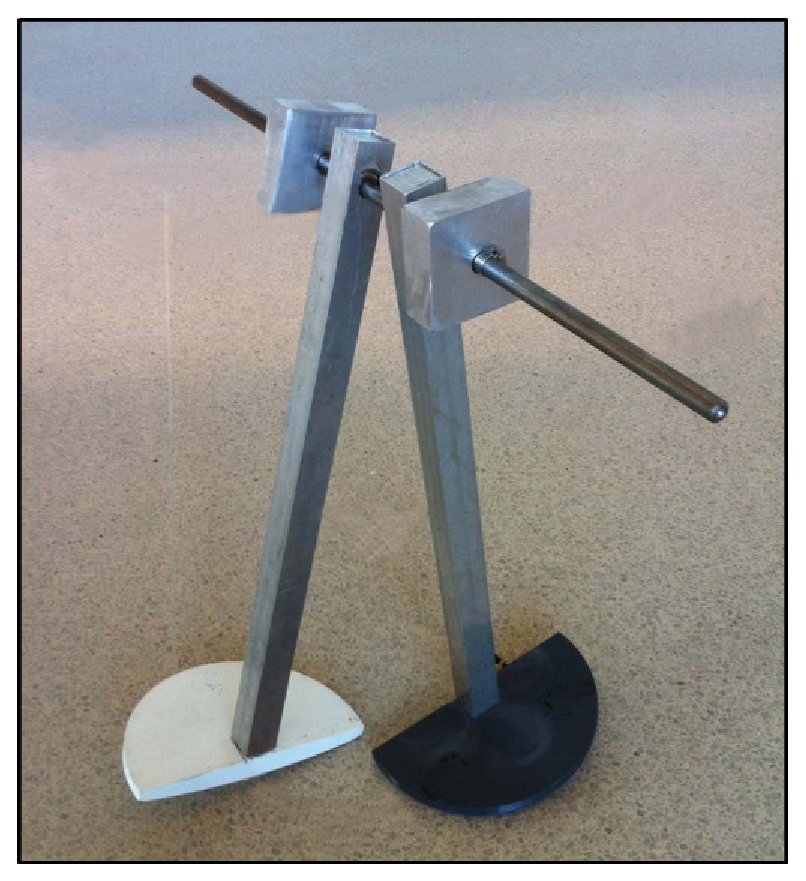
\includegraphics[width=0.26\columnwidth]{compass-gait} \hspace{3em}
  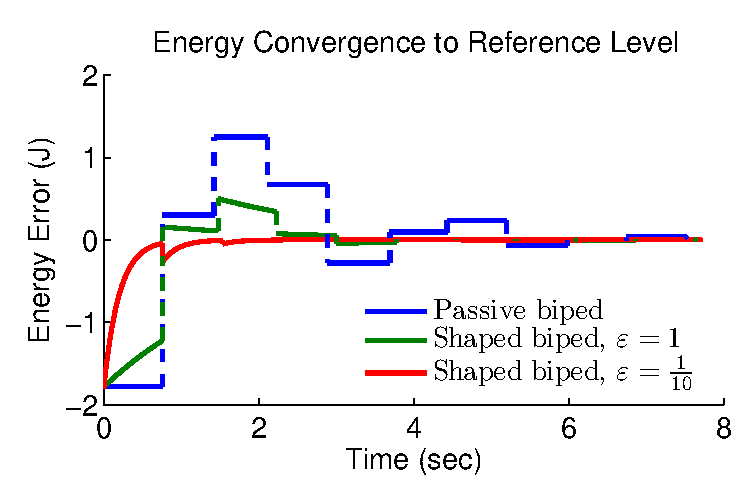
\includegraphics[width=0.45\columnwidth]{cg-energy-comp}
  \caption{Compass-gait biped on a slope (left), energy convergence in
    simulations for passive system and shaped systems with different gains
    (right). Smaller values of $\varepsilon$ result in faster convergence of the energy dynamics.}
  \label{fig:simulation-model}
  \vspace{-1em}
\end{figure}

The development of energy shaping approaches spans the past few decades
although energy-based approaches to analytical mechanics date back over 200
years to the work of Lagrange
% \cite{Lagrange1788}
and the principles of stability involved were first presented by Lyapunov
% \cite{Lyapunov1992}
over 100 years ago.
% 
The ideas herein also build on more recent results spread throughout the literature.
%
Over the last few decades, researchers have presented control schemes which seek
to achieve periodic behaviors in dynamical systems and bipedal walking in
particular by formulating their control objectives in terms of the energy of a
system.
%
Based on McGeer's observation that compass-gait
bipeds\footnote{%
  Video of a compass-gait biped available online
  \href{http://youtu.be/mwugDGGhPmI}{http://youtu.be/mwugDGGhPmI}.%
} with appropriate mass distributions can walk down shallow slopes without
actuation \cite{McGeer1990}, Spong presented controlled symmetries
\cite{Spong2007} as a method for obtaining walking on a compass-gait biped on
flat ground by injecting energy in a such a way that the shaped potential energy
of the robot's gait on flat ground mimicked the potential energy of a passive
biped walking down a slope.
%
% controlled symmetries appeared earlier, but using Spong2007, we can reduce the
% references.
% 
Based on this idea, Spong later provided a controller which could shape the
total energy of a compass-gait biped and showed that the controller would
guarantee asymptotic stability of the energy dynamics to a reference level,
$E_{\mathit{ref}}$, through the continuous dynamics although nothing was
formally established with regards to stability of the overall system.
%
He later demonstrated how the ideas could be extended to non-conservative
systems \cite{Spong2007} by considering energy storage functions.
%
While the compass-gait biped is of interest as a low-dimensional example of
walking, the same method of controlled symmetries has been used as a basis for
achieving walking in more complex models with knees and non-trivial foot action
\cite{Sinnet2009} and has been extended to three-dimensional bipeds using
functional Routhian reduction \cite{Sinnet2009a}.

The energy shaping problem, as formulated herein, falls under a class of
problems involving stability of systems with zero dynamics.
%
In \cite{Ames2014}, a similar problem was considered in which a stabilizing
control law was constructed using control Lyapunov functions to stabilize to a
zero dynamics which exhibited hybrid invariance; that is, for initial conditions
on the intersection of the switching surface and the hybrid zero dynamics
manifold, application of the reset map will result in a state which is still on
the hybrid zero dynamics.
%
This was a key assumption underlying \cite{Ames2014} but this assumption does
not hold for energy shaping as energy is generally not invariant through impact,
though there may be pathological examples which demonstrate this property.
%
In fact, for certain conservative systems like the compass-gait biped, which
exhibits local exponential stability, energy change can only occur through
discrete transitions and so impacts actually act as a stabilizing influence.
%
%Another key difference is the assumption of stability which is necessary for the
%application of energy shaping.
%
%Whereas \cite{Ames2014} requires stability of the system for states restricted
%to the hybrid zero dynamics, this method requires stability of the nominal system
%and does not require hybrid invariance of the zero dynamics.
%
%Thus, while the problems are somewhat similar, they also have their differences
%and are applicable to different types of systems.


%
%The principles involved rely on the well-developed analytical mechanics methods
%of Lagrange as well as the body of literature on stability which centers around
%the ideas presented by Lyapunov.
%
In order to apply energy shaping, one begins with an autonomous hybrid
mechanical system with position and velocity coordinates $(q, {\dot q})$ which
contains a locally exponentially stable periodic orbit, possibly induced by some
feedback control law.
%
For systems of this type, a conserved energy quantity exists through the
continuous dynamics and it comprises kinetic and potential energy as well as an
additional term.
%
This additional term can be treated with a storage function which tracks the
energy flowing out of the system; such energy flow occurs due to
non-conservative forcing.
%
For periodic behaviors, this conserved quantity, expressed as
\begin{align*}
  E_{c} = T(q, {\dot q}) + U(q) - \int_{0}^{t} \! F_{\mathit{nc}}(q(\tau), {\dot
    q}(\tau)) \cdot \frac{dq(\tau)}{d\tau} \ d\tau
\end{align*}
with the terms respectively representing kinetic energy, potential energy, and
stored energy, is also periodic and, by resetting the storage function
appropriately through the discrete dynamics, can be made to be a constant.
%
Using the conserved quantity, which is a function of the system state, and its
constant reference level, one can design an energy shaping controller to drive
the conserved energy of the system to the reference level, thereby stabilizing
the system's energy dynamics.
%
The particular approach discussed achieves this energy stabilization through the
use of a {\em rapidly exponentially stabilizing control Lyapunov function (RES-CLF)} \cite{Ames2014,Freeman1996}.
%
Roughly speaking, one must choose control inputs such that the energy of the
system is exponentially stable through the continuous dynamics.
%
This is done by constructing the Lyapunov candidate function $V(q, {\dot q}) =
(E_{c}(q, {\dot q}) - E_{\mathit{ref}})^{2}$.
%
Because ${\dot V}(q, {\dot q}, u) = L_{f} V(q, {\dot q}) + L_{g} V(q, {\dot
  q}) \, u$ is affine with respect to the control input, the problem can be
posed as a quadratic program operating on a convex set:
\begin{align*}
  \mu_{\varepsilon}(q, {\dot q}) = \argmin_{u \in \mathbb{R}^{m}} & \ u^T \, u\\[-.5em]
  &\hspace{-1.5em}\mbox{s.t. } L_{f} V (q, {\dot q}) + L_{g} V(q, {\dot q}) \, u
  + \frac{c_{3}}{\varepsilon} V(q, {\dot q}) \leq 0.
\end{align*}
This results in an optimal controller that can be evaluated with relatively low
computational cost.
%
In addition to being easy to solve, this formulation confers the added benefit
of allowing torque limitations as well as constraints on friction and on ground
reaction forces, although doing so may destroy feasibility.
%
With no constraints, the solution is feasible and is known in closed form, often
referred to as the pointwise min-norm controller \cite{Freeman1996}.

%In particular, given a hybrid system with an exponentially stable limit
%cycle representing a periodic behavior, the application of energy shaping
%will exponentially stabilize the energy dynamics to a specified reference
%level while maintaining exponential stability of the overall hybrid system.
% 
%The presented control strategy is applicable to a wide class of mechanical
%systems including bipedal locomotion.
% 
%Moreover, the controller involves an optimization problem which is formulated as
%a quadratic program operating on a convex set, thereby permitting the use of
%existing tools for rapidly evaluating the solution.
% 
%Numerical simulations are provided to demonstrate the application and
%usefulness of energy shaping.


In contrast to its predecessors, it has been formally shown that the presented
controller maintains exponential stability of the hybrid system to which it is
applied for small enough control gains.
%
Although formal results regarding the robustness of the shaped system to
perturbations in initial conditions have not yet been established, simulations
show that the method can result in a larger domain of attraction and shorter
stabilization times for limit cycles of certain systems.
%
Indeed simulation results are provided for a cart--spring system to demonstrate
improved convergence properties and for a compass-gait
biped as in Figure~\ref{fig:simulation-model} to
demonstrate the robustness improvement that can be conferred by energy shaping.
%
Despite the lack of formal claims with respect to global properties, the local
stability properties are practically useful when using energy shaping as a
stabilizing controller in operating regions around the desired behavior.
%
Ultimately, the goal will be to apply these methods to complex biped and
humanoid robots with a view toward robotic--assistive devices.

\bibliographystyle{plain}
\bibliography{myrefs}

\end{document}
